% **** Szablon pracy magisterskiej, licencjackiej lub inżynierskiej ****

\documentclass[polish,12pt,twoside,a4paper]{report}

% *************** Definicje stylu dokumentu ***************

% *********************************************************************************
% W pliku tym zdefiniowany jest wygl¹d dokumentu.
% Zmiany tutaj nie s¹ konieczne o ile nie zamierzasz zmieniaæ wygl¹du dokumentu.
% *********************************************************************************

% *************** Za³adowanie pakietów ***************
\usepackage[a4paper,twoside,left=2.0cm,right=1.5cm,top=1.5cm,bottom=1.5cm]{geometry}
\usepackage[T1]{fontenc}
%\usepackage[cp1250]{inputenc}
\usepackage[utf8]{inputenc}
\usepackage[polish]{babel}
\usepackage{amsmath}
\usepackage{amsfonts}
\usepackage{graphicx}
\usepackage{graphics}
\usepackage{times}
\usepackage{indentfirst}%wciecia a nowych akapitach
\usepackage{listings}
\usepackage{url}
\usepackage[colorlinks=true, linkcolor=black, urlcolor=black, citecolor=black]{hyperref}

\selectlanguage{polish}

%szerokoœœ wciêæ
\setlength{\parindent}{1.25cm}

%numeracja stron
\usepackage{fancyhdr}
\pagestyle{fancy}
\fancyhf{} % usun biezace ustawienia pagin
\fancyhead[LE,RO]{ }
\fancyhead[LO]{ }
\fancyhead[RE]{ }
\fancyfoot[LE,RO]{\small\thepage}
\fancyfoot[LO]{ }
\fancyfoot[RE]{ }
\renewcommand{\headrulewidth}{0.0pt}
\renewcommand{\footrulewidth}{0.0pt}
\addtolength{\headheight}{0.0pt} % pionowy odstep na kreske
\fancypagestyle{plain}{%
\fancyhead{} % usun p. górne na stronach pozbawionych
% numeracji (plain)
\renewcommand{\headrulewidth}{0.0pt} % pozioma kreska
}

% *************** Definicje niektórych kolorów ***************
\usepackage{color}

\definecolor{greenyellow}   {cmyk}{0.15, 0   , 0.69, 0   }
\definecolor{yellow}        {cmyk}{0   , 0   , 1   , 0   }
\definecolor{goldenrod}     {cmyk}{0   , 0.10, 0.84, 0   }
\definecolor{dandelion}     {cmyk}{0   , 0.29, 0.84, 0   }
\definecolor{apricot}       {cmyk}{0   , 0.32, 0.52, 0   }
\definecolor{peach}         {cmyk}{0   , 0.50, 0.70, 0   }
\definecolor{melon}         {cmyk}{0   , 0.46, 0.50, 0   }
\definecolor{yelloworange}  {cmyk}{0   , 0.42, 1   , 0   }
\definecolor{orange}        {cmyk}{0   , 0.61, 0.87, 0   }
\definecolor{burntorange}   {cmyk}{0   , 0.51, 1   , 0   }
\definecolor{bittersweet}   {cmyk}{0   , 0.75, 1   , 0.24}
\definecolor{redorange}     {cmyk}{0   , 0.77, 0.87, 0   }
\definecolor{mahogany}      {cmyk}{0   , 0.85, 0.87, 0.35}
\definecolor{maroon}        {cmyk}{0   , 0.87, 0.68, 0.32}
\definecolor{brickred}      {cmyk}{0   , 0.89, 0.94, 0.28}
\definecolor{red}           {cmyk}{0   , 1   , 1   , 0   }
\definecolor{orangered}     {cmyk}{0   , 1   , 0.50, 0   }
\definecolor{rubinered}     {cmyk}{0   , 1   , 0.13, 0   }
\definecolor{wildstrawberry}{cmyk}{0   , 0.96, 0.39, 0   }
\definecolor{salmon}        {cmyk}{0   , 0.53, 0.38, 0   }
\definecolor{carnationpink} {cmyk}{0   , 0.63, 0   , 0   }
\definecolor{magenta}       {cmyk}{0   , 1   , 0   , 0   }
\definecolor{violetred}     {cmyk}{0   , 0.81, 0   , 0   }
\definecolor{rhodamine}     {cmyk}{0   , 0.82, 0   , 0   }
\definecolor{mulberry}      {cmyk}{0.34, 0.90, 0   , 0.02}
\definecolor{redviolet}     {cmyk}{0.07, 0.90, 0   , 0.34}
\definecolor{fuchsia}       {cmyk}{0.47, 0.91, 0   , 0.08}
\definecolor{lavender}      {cmyk}{0   , 0.48, 0   , 0   }
\definecolor{thistle}       {cmyk}{0.12, 0.59, 0   , 0   }
\definecolor{orchid}        {cmyk}{0.32, 0.64, 0   , 0   }
\definecolor{darkorchid}    {cmyk}{0.40, 0.80, 0.20, 0   }
\definecolor{purple}        {cmyk}{0.45, 0.86, 0   , 0   }
\definecolor{plum}          {cmyk}{0.50, 1   , 0   , 0   }
\definecolor{violet}        {cmyk}{0.79, 0.88, 0   , 0   }
\definecolor{royalpurple}   {cmyk}{0.75, 0.90, 0   , 0   }
\definecolor{blueviolet}    {cmyk}{0.86, 0.91, 0   , 0.04}
\definecolor{periwinkle}    {cmyk}{0.57, 0.55, 0   , 0   }
\definecolor{cadetblue}     {cmyk}{0.62, 0.57, 0.23, 0   }
\definecolor{cornflowerblue}{cmyk}{0.65, 0.13, 0   , 0   }
\definecolor{midnightblue}  {cmyk}{0.98, 0.13, 0   , 0.43}
\definecolor{navyblue}      {cmyk}{0.94, 0.54, 0   , 0   }
\definecolor{royalblue}     {cmyk}{1   , 0.50, 0   , 0   }
\definecolor{blue}          {cmyk}{1   , 1   , 0   , 0   }
\definecolor{cerulean}      {cmyk}{0.94, 0.11, 0   , 0   }
\definecolor{cyan}          {cmyk}{1   , 0   , 0   , 0   }
\definecolor{processblue}   {cmyk}{0.96, 0   , 0   , 0   }
\definecolor{skyblue}       {cmyk}{0.62, 0   , 0.12, 0   }
\definecolor{turquoise}     {cmyk}{0.85, 0   , 0.20, 0   }
\definecolor{tealblue}      {cmyk}{0.86, 0   , 0.34, 0.02}
\definecolor{aquamarine}    {cmyk}{0.82, 0   , 0.30, 0   }
\definecolor{bluegreen}     {cmyk}{0.85, 0   , 0.33, 0   }
\definecolor{emerald}       {cmyk}{1   , 0   , 0.50, 0   }
\definecolor{junglegreen}   {cmyk}{0.99, 0   , 0.52, 0   }
\definecolor{seagreen}      {cmyk}{0.69, 0   , 0.50, 0   }
\definecolor{green}         {cmyk}{1   , 0   , 1   , 0   }
\definecolor{forestgreen}   {cmyk}{0.91, 0   , 0.88, 0.12}
\definecolor{pinegreen}     {cmyk}{0.92, 0   , 0.59, 0.25}
\definecolor{limegreen}     {cmyk}{0.50, 0   , 1   , 0   }
\definecolor{yellowgreen}   {cmyk}{0.44, 0   , 0.74, 0   }
\definecolor{springgreen}   {cmyk}{0.26, 0   , 0.76, 0   }
\definecolor{olivegreen}    {cmyk}{0.64, 0   , 0.95, 0.40}
\definecolor{rawsienna}     {cmyk}{0   , 0.72, 1   , 0.45}
\definecolor{sepia}         {cmyk}{0   , 0.83, 1   , 0.70}
\definecolor{brown}         {cmyk}{0   , 0.81, 1   , 0.60}
\definecolor{tan}           {cmyk}{0.14, 0.42, 0.56, 0   }
\definecolor{gray}          {cmyk}{0   , 0   , 0   , 0.50}
\definecolor{black}         {cmyk}{0   , 0   , 0   , 1   }
\definecolor{white}         {cmyk}{0   , 0   , 0   , 0   } 

% *************** Koniec definicji stylu dokumentu ***************


%definicja przydatnych poleceń
\newcommand{\wydzial}{KOLEGIUM INFORMATYKI STOSOWANEJ}
\newcommand{\kierunek}{Kierunek: INFORMATYKA}
\newcommand{\specjalnosc}{Specjalność: Inżynieria Danych}
\newcommand{\autor}{Norbert Świerczek}
\newcommand{\album}{Nr albumu studenta w67201}
\newcommand{\temat}{System do zarządzania dokumentami w firmie}
\newcommand{\promotor}{mgr inż. Ewa Żesławska}
\newcommand{\typpracy}{Praca projektowa programowanie obiektowe C\#}
\newcommand{\miasto}{Rzeszów}
\newcommand{\rok}{2024}

\begin{document}

% *************** Włączenie definicji pierwszych stron ***************
% *************** Strony tytułowe ***************

% ************************************************************
% W tym miejscu znajduje sie definicja wyglądu pierwszych stron:
% strony tytułowej, strony z oświadczeniem o treści pracy
% i strony ze spisem treści
% ************************************************************
% *************** Strona tytułowa ***************
%umieszczenie logo i nazwy uczelni
\noindent
\parbox{65mm}{
\includegraphics[width=13.0cm, height=3.0cm]{logoWSIiZ}}

\vspace{10mm}
\begin{center}
{\Large{}\textbf{\wydzial}}
\end{center}
\vspace{10mm}
\noindent
\hspace{30mm}{\Large{}\textbf{\kierunek}}\\

\noindent
\hspace{30mm}{\Large{}\textbf{\specjalnosc}}
\vspace{30mm}
\begin{center}
	{\large{}\autor}\\
	{\large{}\album}\\
	\vspace{15pt}
	{\huge{}\textbf{\textit{\temat}}}\\
	\vspace{20pt}
	{\normalsize{}Prowadzący: \promotor}\\
	\vspace{100pt}
	{\LARGE{}\textbf{\typpracy}}\\
	\vspace{190pt}
	{\large{}\textbf{\miasto {} \rok}}
\end{center}

% pusta zawartość stopki - brak numeru strony
\thispagestyle{empty}

% *************** Strona z oświadczeniem o treści pracy ***************
\newpage
\text{}

\thispagestyle{empty}
\newpage


% *************** Spis treści ***************
\tableofcontents
% pusta zawartość stopki - brak numeru strony
\thispagestyle{empty}
\newpage

% *************** Koniec pliku front.tex ***************



% *************** Część główna pracy ***************
\chapter*{Wstęp}

Współczesne organizacje funkcjonują w środowisku, w którym skuteczne zarządzanie dokumentami staje się kluczowe dla zapewnienia efektywności pracy oraz przestrzegania przepisów prawnych. W miarę jak firmy rozwijają się i generują coraz większe ilości dokumentów, konieczne staje się wdrożenie nowoczesnych narzędzi, które pozwolą na sprawne zarządzanie obiegiem informacji. Tradycyjne metody obiegu dokumentów, oparte na papierze, są czasochłonne, podatne na błędy i opóźnienia, a także ograniczają dostępność danych. W związku z tym, coraz więcej firm decyduje się na wdrożenie systemów informatycznych, które usprawniają zarządzanie dokumentami, umożliwiając łatwe ich tworzenie, edytowanie, archiwizowanie i usuwanie.

Projekt, którego celem jest stworzenie systemu informatycznego do zarządzania dokumentami w firmie, odpowiada na rosnącą potrzebę automatyzacji tych procesów. System ten ma na celu uproszczenie obiegu dokumentów, zapewniając jednocześnie pełną kontrolę nad ich tworzeniem, przechowywaniem oraz dostępem. Dzięki wdrożeniu nowoczesnego systemu, pracownicy będą mogli szybko i bezpiecznie zarządzać dokumentami, a firma będzie mogła skutecznie przestrzegać obowiązujących regulacji prawnych dotyczących przechowywania i archiwizowania dokumentów.

Aplikacja pozwoli na łatwe tworzenie, edytowanie oraz archiwizowanie dokumentów, zapewniając przejrzystość w obiegu informacji w firmie. Dodatkowo, system umożliwi tworzenie kategorii dokumentów, co ułatwi organizację materiałów i szybki dostęp do niezbędnych informacji. Ważnym aspektem będzie również funkcjonalność związana z usuwaniem dokumentów, umożliwiająca ich bezpieczne usunięcie, zgodnie z wymaganiami prawnymi dotyczącymi przechowywania danych.

\addcontentsline{toc}{chapter}{Wstęp}
\newpage
% ********** Rozdział 1 **********
\chapter{Opis założeń projektu}

\section{Cele projektu}
Celem projektu jest stworzenie systemu informatycznego wspierającego zarządzanie dokumentami w firmie. System ma na celu usprawnienie obiegu dokumentów, umożliwiając ich łatwe tworzenie, edytowanie, archiwizowanie oraz usuwanie. Zaimplementowane funkcje mają zapewnić pełną kontrolę nad dokumentami w firmie, umożliwiając pracownikom szybki dostęp do niezbędnych materiałów, a także ich bezpieczne przechowywanie.

System ma zapewnić możliwość tworzenia, edytowania, usuwania dokumentów oraz ich archiwizowania, umożliwiając pracownikom szybsze zarządzanie dokumentacją, jak również zapewnienie zgodności z procedurami firmowymi dotyczącymi obiegu dokumentów.

\section{Wymagania funkcjonalne i niefunkcjonalne}

\noindent \textbf{Wymagania funkcjonalne}

\begin{itemize}
    \item System musi umożliwiać tworzenie, edytowanie, archiwizowanie oraz usuwanie dokumentów.
    \item Użytkownicy powinni mieć możliwość przeglądania szczegółowych informacji o dokumentach, takich jak data utworzenia, autor, status oraz historia zmian.
    \item System powinien pozwalać na tworzenie i zarządzanie kategoriami dokumentów, co ułatwi ich klasyfikację oraz szybkie wyszukiwanie.
    \item System powinien umożliwiać przypisywanie uprawnień do dokumentów, aby kontrolować dostęp do wrażliwych materiałów (np. tylko wybrani użytkownicy będą mogli edytować lub usuwać dokumenty).
\end{itemize}

\noindent \textbf{Wymagania niefunkcjonalne}

\begin{itemize}
    \item System musi charakteryzować się wysoką wydajnością, zapewniając płynne przetwarzanie dużych zbiorów dokumentów i umożliwiając szybkie wyszukiwanie.
    \item Powinien być skalowalny, umożliwiając łatwą rozbudowę systemu i dodawanie nowych funkcji w miarę rozwoju firmy.
    \item Interfejs użytkownika powinien być intuicyjny i łatwy w obsłudze, aby zapewnić szybkie wdrożenie pracowników oraz bezproblemowe korzystanie z systemu.
    \item System musi być kompatybilny z popularnymi systemami operacyjnymi.
    \item Należy zapewnić odpowiedni poziom bezpieczeństwa danych, w tym szyfrowanie danych i ochrona przed nieautoryzowanym dostępem.
\end{itemize}

% ********** Koniec rozdziału **********

\newpage
% ********** Rozdział 2 **********
\chapter{Opis struktury projektu}

\section{Opis Struktury Projektu}
System zarządzania dokumentami został zaprojektowany w języku \textbf{C\#}, wykorzystując programowanie obiektowe (OOP). Struktura projektu składa się z kilku głównych klas, które odpowiadają za przechowywanie, zarządzanie i przetwarzanie dokumentów.


\subsection{Diagram Klas}
Poniżej przedstawiono diagram klas ilustrujący hierarchię obiektów w systemie:

\begin{center}
    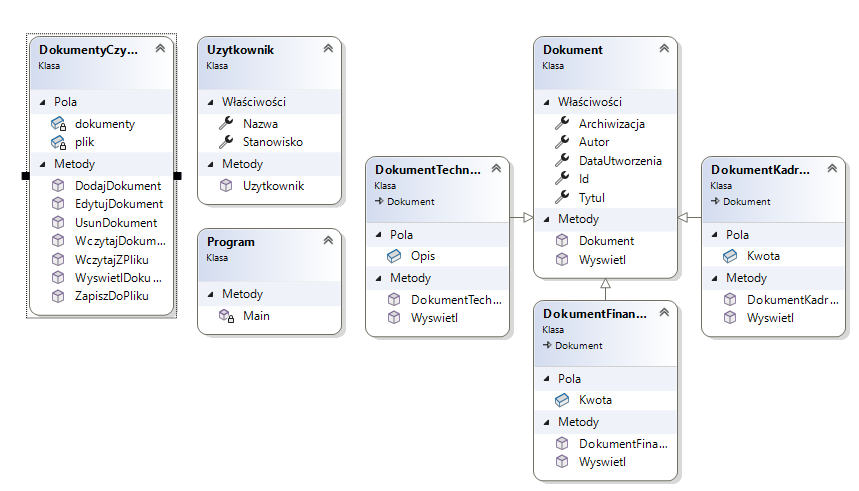
\includegraphics[width=0.8\textwidth]{diagramklas.png}
\end{center}


\subsection{Klasa bazowa: Dokument}
\begin{itemize}
\item Właściwości: \texttt{Id}, \texttt{Tytul}, \texttt{Autor}, \texttt{DataUtworzenia}, \texttt{CzyZarchiwizowany}
\item Metoda abstrakcyjna: \texttt{WyswietlInformacje()}
\end{itemize}

\subsection{Klasy pochodne:}
\begin{itemize}
\item \textbf{DokumentFinansowy} (\texttt{Kwota} jako dodatkowa właściwość)
\item \textbf{DokumentKadrowy} (\texttt{Pracownik} jako dodatkowa właściwość)
\item \textbf{DokumentTechniczny} (\texttt{Opis} jako dodatkowa właściwość)
\end{itemize}

\subsection{Klasa Użytkownik}
\begin{itemize}
\item Właściwości: \texttt{Nazwa}, \texttt{Rola}
\item Reprezentuje użytkowników z różnymi uprawnieniami (Administrator, Pracownik, Gość)
\end{itemize}

\subsection{Klasa DokumentyCzynnosci}
\begin{itemize}
\item Metody:
\begin{itemize}
\item {DodajDokument}\texttt{(Dokument dokument, Użytkownik użytkownik)}
\item {UsunDokument}\texttt{(int id, Użytkownik użytkownik)}
\item {EdytujDokument}\texttt{(int id, string nowyTytul, string nowyAutor, bool nowaArchiwizacja, Użytkownik użytkownik)}
\item {WczytajZPliku()}
\item {ZapiszDoPliku()}
\item {WyswietlDokumenty()}
\end{itemize}
\end{itemize}

\subsection{Klasa Program (obsługa interfejsu użytkownika)}
\begin{itemize}
\item Menu umożliwiające wybór operacji na dokumentach
\item Wczytywanie danych przy starcie aplikacji
\item Obsługa logowania użytkownika
\end{itemize}

\section{Opis Techniczny}
\subsection{Język Programowania i Narzędzia}
Projekt został napisany w języku \textbf{C\#} w środowisku \textbf{Microsoft Visual Studio 2022}. 

\subsection{Minimalne Wymagania Sprzętowe}
\begin{itemize}
    \item Procesor: Intel Core i3 lub wyższy
    \item Pamięć RAM: 4 GB
    \item System operacyjny: Windows 10/11
    \item Dysk: Minimum 200 MB wolnej przestrzeni
\end{itemize}

\section{Zarządzanie Danymi i Baza Danych}
Dane są przechowywane w pliku tekstowym \texttt{dokumenty.txt}. Każdy dokument jest zapisywany w postaci linii danych oddzielonych separatorem \texttt{|}






% ********** Koniec rozdziału **********

\newpage
% ********** Rozdział 4 **********
\chapter{Harmonogram realizacji projektu}


\section{Harmonogram Realizacji Projektu}
Plan realizacji projektu przedstawiono na diagramie Gantta:

\begin{center}
    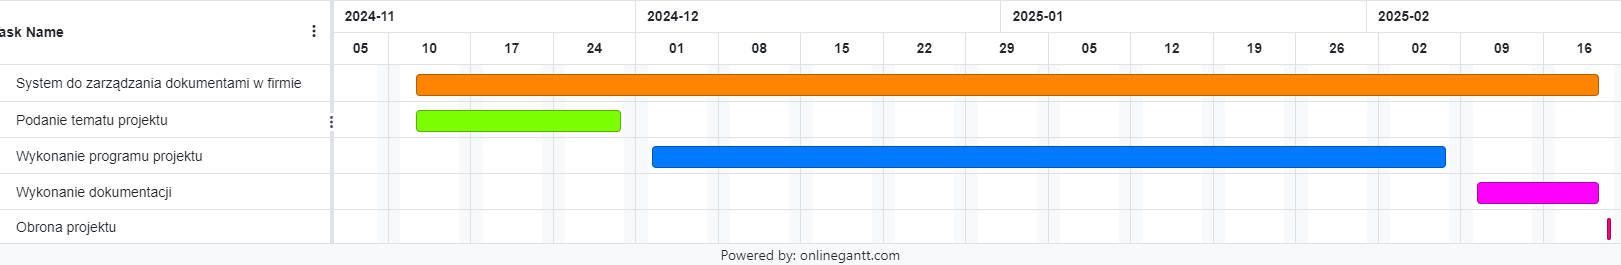
\includegraphics[width=1\textwidth]{gantt.png}
\end{center}

\begin{itemize}
    \item \textbf{Podanie tematu projektu} (listopad 2024)
    \item \textbf{Wykonanie programu projektu} (grudzień 2024 – styczeń 2025)
    \item \textbf{Wykonanie dokumentacji} (luty 2025)
    \item \textbf{Obrona projektu} (ostatni tydzień lutego 2025)
\end{itemize}

\section{Repozytorium i system kontroli wersji}

Projekt jest zarządzany za pomocą systemu kontroli wersji \textbf{Git}, a kod jest przechowywany w repozytorium \textbf{GitHub}. 

Repozytorium projektu jest dostępne pod adresem:
\href{https://github.com/NorbertSwierczek/P-L_Programowanie-obiektowe_3IIZ-2023-GPL02/tree/main/projekt}{github.com/NorbertSwierczek}

% ********** Koniec rozdziału **********

\newpage
% ********** Rozdział 4 **********
\chapter{Prezentacja warstwy użytkowej projektu}

\section{Opis interfejsu użytkownika}

\begin{figure}[htbp]
  \centering
  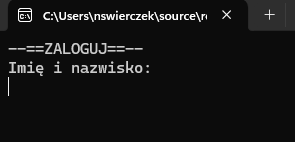
\includegraphics[width=0.6\textwidth]{zalog.png}
  \caption{Panel logowania}
  \label{fig:zalog}
\end{figure}

\begin{figure}[htbp]
  \centering
  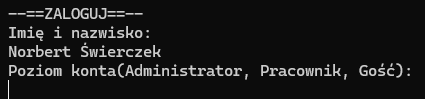
\includegraphics[width=0.6\textwidth]{zalog2.png}
  \caption{Wybór poziomu konta}
  \label{fig:zalog2}
\end{figure}

\begin{figure}[htbp]
  \centering
  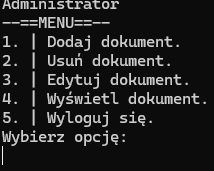
\includegraphics[width=0.6\textwidth]{menu.png}
  \caption{Główne menu systemu z opcjami CRUD (tworzenie, edycja, usuwanie, przeglądanie dokumentów) oraz możliwością wylogowania}
  \label{fig:menu}
\end{figure}

\begin{figure}[htbp]
  \centering
  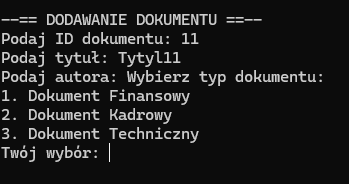
\includegraphics[width=0.7\textwidth]{dodawanie.png}
  \caption{Proces dodawania nowego dokumentu z wyborem typu (Finansowy/Kadrowy/Techniczny) i specjalnym polem kwoty dla dokumentów finansowych}
  \label{fig:dodawanie}
\end{figure}

\begin{figure}[htbp]
  \centering
  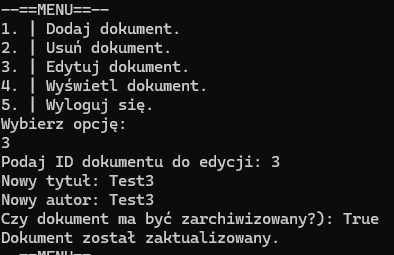
\includegraphics[width=0.7\textwidth]{edytuj.png}
  \caption{Edycja istniejącego dokumentu z możliwością zmiany tytułu, autora oraz statusu archiwizacji}
  \label{fig:edycja}
\end{figure}

\begin{figure}[htbp]
  \centering
  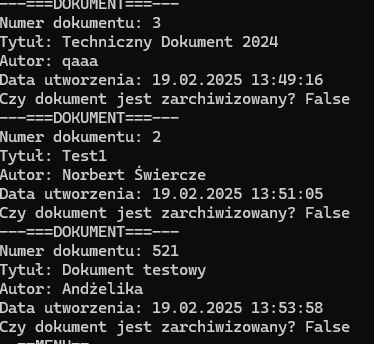
\includegraphics[width=0.8\textwidth]{wyswietl.png}
  \caption{Przeglądanie dokumentów ze szczegółowymi informacjami: ID, tytuł, autor, data utworzenia i status archiwizacji}
  \label{fig:przegladanie}
\end{figure}

\begin{figure}[htbp]
  \centering
  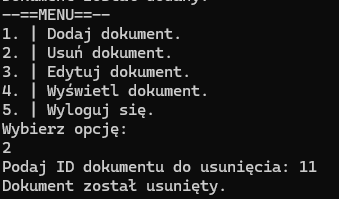
\includegraphics[width=0.6\textwidth]{usun.png}
  \caption{Mechanizm usuwania dokumentów po podaniu identyfikatora z potwierdzeniem operacji}
  \label{fig:usuwanie}
\end{figure}


% ********** Koniec rozdziału **********

\newpage
% ********** Rozdział 4 **********
\chapter{Podsumowanie}

\section{Podsumowanie}
Projekt „System do zarządzania dokumentami w firmie” to aplikacja w {C\#} umożliwiająca dodawanie, edytowanie i przeglądanie dokumentów z kontrolą dostępu użytkowników. System wykorzystuje pliki tekstowe do przechowywania danych, z możliwością przyszłej integracji z bazą SQL.

Zastosowano programowanie obiektowe (OOP) oraz system kontroli wersji Git z repozytorium na GitHubie. Harmonogram realizacji projektu został zaplanowany za pomocą diagramu Gantta.

Projekt spełnił swoje założenia i stanowi solidną bazę do dalszego rozwoju, np. o interfejs graficzny czy integrację z nowoczesnymi bazami danych.



% ********** Koniec rozdziału **********


\newpage

% *************** Bibliografia ***************
\begin{thebibliography}{6}
\addcontentsline{toc}{chapter}{Bibliografia}
%dodanie wpisu do spisu bibliograficznego

\bibitem{www-1} https://www.businessnewsdaily.com/15605-document-management-system-benefits.html
\bibitem{www-2} https://www.jstor.org/stable/40012822
\bibitem{www-3} https://pl.wikipedia.org/wiki/DiagramGantta
\bibitem{www-4} https://monday.com/ap/gantt
\bibitem{www-5} https://www.overleaf.com
\end{thebibliography}
\newpage

% *************** Zakończenie ***************
% *************** Zakończenie ***************

%***************************************************************************************
% W tym miejscu znajdują się polecenia odpowiedzialne za tworzenie
% spisu ilustracji, spisu treści oraz streszczenia pracy
%***************************************************************************************

%spis rysunków
\addcontentsline{toc}{chapter}{Spis rysunków}
\listoffigures
\newpage

%spis tablic
\addcontentsline{toc}{chapter}{Spis tablic}
\listoftables
\newpage

% %streszczenie
% \addcontentsline{toc}{chapter}{Streszczenie}
% \noindent
% {\footnotesize{}\textbf{Wyższa Szkoła Informatyki i Zarządzania z siedzibą w Rzeszowie\\
% Kolegium Informatyki Stosowanej}
% \vspace{30pt}

% \begin{center}
% \textbf{Streszczenie pracy dyplomowej inżynierskiej}\\
% \temat
% \end{center}

% \vspace{30pt}
% \noindent
% \textbf{Autor: \autor
% \\Promotor: \promotor
% \\Słowa kluczowe: tutaj umieść słowa kluczowe}
% \vspace{40pt}
% \\Treść streszczenia, czyli kilka zdań dotyczących treści pracy dyplomowej w języku polskim.
% \vspace{80pt}

% \noindent
% \textbf{The University of Information Technology and Management in Rzeszow\\
% Faculty of Applied Information Technology}
% \vspace{30pt}

% \begin{center}
% \textbf{Thesis Summary\\}
% Tytuł pracy w języku angielskim
% \end{center}

% \vspace{30pt}
% \noindent
% \textbf{Author: \autor
% \\Supervisor: \promotor
% \\Key words: tutaj umieść słowa kluczowe}
% \vspace{40pt}
% \\Treść streszczenia, czyli kilka zdań dotyczących treści pracy dyplomowej w języku angielskim - tłumaczenie tekstu z języka polskiego.
% }

% *************** Koniec pliku back.tex ***************


\end{document}
% *************** Koniec pliku szablon.tex ***************
